\documentclass[a4paper,12pt]{article}

% Paquetes
\usepackage[utf8]{inputenc}
\usepackage{graphicx}
\usepackage{amsmath, amssymb}
\usepackage[margin = 1in]{geometry}
\usepackage[spanish, es-tabla]{babel}
\spanishdecimal{.}
\usepackage{color}
\usepackage{hyperref}

\usepackage{inconsolata}
\usepackage{listings}
\usepackage{xcolor}

\lstset{
    language=C,
    basicstyle=\ttfamily\scriptsize,
    numbers=left,
    numberstyle=\tiny,
    numbersep=5pt,
    %backgroudcolor={gray!10},
    keywordstyle=\color{blue},
    commentstyle=\color{gray},
    stringstyle=\color{red},
    showstringspaces=false,
    frame=single,
    breaklines=true,
    tabsize=2,
    captionpos=t,
    extendedchars=true,
    literate={á}{{\'a}}1 {é}{{\'e}}1 {í}{{\'i}}1 {ó}{{\'o}}1 {ú}{{\'u}}1 {Ú}{{\'U}}1 {ñ}{{\~{n}}}1 {°}{{$^{\circ}$}}1
}

% Comandos
\newcommand{\R}{\mathbb{R}}
\newcommand{\Z}{\mathbb{Z}}
\newcommand{\N}{\mathbb{N}}
\newcommand{\var}{\operatorname{Var}}
\newcommand{\cov}{\operatorname{Cov}}
\newcommand{\E}{\mathbb{E}}
\newcommand{\norm}[1]{\left\Vert#1\right\Vert}

\renewcommand{\O}{\mathcal{O}}
\renewcommand{\P}{\mathbb{P}}

% Título
\title{Física computacional - Modelo de Ising \\ Laboratorio 4}
\author{El mono}
\date{}

% Documento
\begin{document}

\maketitle

\begin{abstract}
    Simulamos el modelo de Ising y calculamos algunas variables termodinámicas usando el método de Metropolis. Estudiamos la dependencia de estas variables con respecto a la temperatura del sistema y, en particular, observamos que existe una temperatura crítica $T_c$ en la cual la magnetización presenta una bifurcación. Esto es, una transición de fase.
\end{abstract}

\section{Introducción}

En este trabajo simulamos el modelo de Ising y calculamos algunas variables termodinámicas usando Markov Chain Monte Carlo (MCMC) con una cadena generada mediante el método Metropolis \cite{metropolis1953equation}. Concretamente, simulamos un toro discreto de $n^2$ partículas, cada una de las cuales puede tener spin {\it up} o {\it down}; y calculamos, en función de la temperatura $T^*$ (reducida) la magnetización $M$, la energía $E$, la susceptibilidad $\chi$, el calor específico $C$ y la temperatúra crítica $T_c$. Estos cálculos son, en general, de la forma
\begin{equation}
    \label{eq:ejemplo}
    Q = \E(f_Q(X)),
\end{equation}
donde $X : \Omega \to S$ es una variable aleatoria que cae en el espacio $S$ de esatados del sistema con distribución de Boltzmann, y $f_Q : S \to \R$ es alguna función por medio de la cual se calcula la cantidad $Q$.\\

Dado que el espacio de estados $S$  es de cardinal $2^{n^2}$ (pues cada una de las $n^2$ partículas puede tener spin {\it up} o {\it down}), es demasiado costoso calcular $Q$ por definición. Por esta razón usualmente se opta por aproximar $Q$ mediante integración Monte Carlo (MC). Sin embargo, no es trivial implementar este método de integración sobre $S$ (pensándolo como un espacio de probabilidad con la distribución de Boltzmann). Una cantidad considerable de teoría de probabilidades es necesaria para entender (al menos, superficielmente) por qué funciona esta técnica y cuáles son sus limitaciones. En la siguiente sección presentamos un poco de esta teoría (para más detalle, ver \cite{janke2009statistical,schachinger2007mcmc}).

\section{Preliminares}
\label{sec:preliminares}

En esta sección explicamos brevemente el método de Metrópolis y su utilidad en el contexto de la integración Monte Carlo. Esto es porque creemos que conocer ciertos detalles de la teoría de probabilidades puede ayudar a entender algunos de los fenómenos que se observan más adelante en las simulaciones numéricas.

\subsection{Monte Carlo Markov Chain}

Recordemos que la integración MC para calcular \eqref{eq:ejemplo} requiere una forma de muestrear $X$, esto es, una forma de generar una sucesión de estados que sean realizaciones de variables $X_n$ independientes e idénticamente distribuídas con la distribución de $X$. Hay varias formas de hacer esto, una de ellas consiste en generar una cadena de Markov tal que sus variables se aproximen a una muestra de $X$. De aquí el nombre: {\it Markov Chain Monte Carlo}.\\

Supongamos que existe una cadena de Markov $Y = (Y_n)$ sobre $S$ con una única distribución invariante $\pi$ igual a la distribución deseada (en este caso, la distribución de Boltzmann). Entonces, independientemente de la distribución inicial (generalmente $Y_0$ es uniforme o atómica), $Y_n$ converge debilmente\footnote{Esto es, $\E(h(Y_n)) \to \E(h(X))$ para toda $h$ continua y acotada.} a $X$. Así, a partir de cierto $N \in \N$, la cadena $Z = (Y_{N + n})$ se distribuye aproximadamente $\pi$. El fragmento restante de la cadena: $Y_0, Y_1, \dots, Y_{N - 1}$ se llama el {\it burn-in} y se descarta.

Ahora, si bien $Z$ es un proceso de Markov donde cada $Z_n$ se distribuye aproximadamente $\pi$, los $Z_n$ podrían no ser independientes (recordemos que estamos en busca de una muestra de $X$, para lo cual la independencia es un factor crucial). En estas circunstancias es necesario extender la teoría de integración MC al caso MCMC con muestreo no independiente y calcular nuevamente la varianza de la integral. En este trabajo no discutimos estos cálculos, simplemente mencionamos que la varianza de la integral MC es ahora inversamente proporcional al número de muestras (como antes) y proporcional a $\tau_a$, una variable llamada tiempo de autocorrelación que representa, intuitivamente, cuantas muestras $Z_n$ debemos descartar para emular un muestreo independiente. En otras palabras, $\tau_a$ se define de forma que el proceso
\begin{equation*}
    W = (Z_0, Z_{\tau_a}, Z_{2\tau_a}, \dots)
\end{equation*}
no presente evidencia de dependencia.\\

Sobre el final del trabajo estimaremos algunos tiempos de autocorrelación mediante la ecuación (ver \cite{janke2009statistical, schachinger2007mcmc})
\begin{equation}
    \label{eq:tiempo_de_autocorrelacion}
    \tau_a = \dfrac{1}{2} + \sum_{k \in \N} A(k),
\end{equation}
donde
\begin{equation}
    \label{eq:autocorrelacion}
    A(k) = \dfrac{\cov (f_Q(Z_0), f_Q(Z_k))}{\var (f_Q(Z_0))} = \dfrac{\E(f_Q(Z_0)f_Q(Z_k)) - \E^2(f_Q(Z_n))}{\E((f_Q(Z_0))^2) - \E^2(f_Q(Z_n))}
\end{equation}
es la función de autocorrelación del proceso $f_Q(Z)$ y depende de la variable termodinámica $Q$ que estemos estimando.

\subsection{Método de Matropolis}

Una forma ampliamente utilizada para construir una cadena de Markov con distribución invariante dada (en nuestro caso, la distribución de Boltzmann) es el método de Metropolis-Hastings. Este método define una cadena \( (Y_n) \) sobre el espacio de estados \( S \) a partir de una \emph{propuesta} de transición, esto es, una familia de distribuciones de probabilidad \( g(x' \mid x) \), que especifica la probabilidad de proponer un nuevo estado \( x' \in S \) dado el estado actual \( x \in S \).\footnote{Formalmanete, se especifica una familia de medidas de probabilidad indexadas por $S$, pero por consistencia con la bibliografía, denotamos esta familia por medio de sus funciones densidad condicional $g(\; \cdot \mid x)$ a pesar de que no necesariamente son absolutamente continuas con respecto a la medida de Lebesgue.} A partir del estado actual \( Y_n = x \), se genera un candidato \( x' \sim g(\; \cdot \mid x) \), el cual es aceptado con probabilidad
\begin{equation}
    \label{eq:p_aceptacion}
    \P(\text{aceptar } x' \mid x) = \min \left\{1, \frac{\pi(x')\, g(x \mid x')}{\pi(x)\, g(x' \mid x)} \right\},
\end{equation}
y rechazado (manteniendo el estado actual \( Y_{n+1} = x \)) con la probabilidad complementaria. Este procedimiento garantiza que la cadena resultante sea reversible con respecto a \( \pi \) y, bajo ciertas condiciones, ergódica. En particular, el método prouesto originalmente por Metropolis consideraba únicamente familias de distribuciones simétricas. Esto es, $g(x \mid x') = g(x' \mid x)$, de forma que la ecuación \eqref{eq:p_aceptacion} se simplifica.\\

Será importante notar el siguiente comportamiento en el método de Metropolis. Hemos dicho que a partir de un estado $Y_n = x$ se muestrea (con distribución $g(\; \cdot \mid x)$) un nuevo punto, al que más tarde decidiremos si movernos o no (con probabilidad dada por \eqref{eq:p_aceptacion}). Intuitivamente, la sucesión $Y_n$ navega por $S$ pegando saltos de longitud dada por $g$. ¿Qué ocurre si la distribución invariante $\pi$ es, por poner un ejemplo, bimodal con dos regiones de alta probabilidad separadas por un valle de baja probabilidad? Si $g$ tiene poca varianza e $Y_n = x$ se encuentra en una de las regiones de alta probabilidad, es poco probable que {\it salte} hacia la otra region. Si bien está garantizado (por la convergencia debil) que eventualmente $Y_n$ saltará hacia la otra región, en un experimento numérico, esto puede demorar mucho. Es posible que al hacer MCMC con este tipo de distribuciones, la realización de $Y_n$ que usemos no represente $\pi$ (como queremos) sinó la restricción de $\pi$ a una de estas regiones.\\

En resumen, el método de Metropolis es una forma de generar una cadena de Markov con la cual se aproxima una muestra de una distribución $\pi$. Con esta muestra se calcula la integral MC. Entre las limitaciones más importantes de esta técnica tenemos que: debemos descartar el {\it burn in}, cuyo tamaño es desconocido y difícil de acotar eficientemente, no tenemos independencia, aunque podemos simularla conociendo $\tau_a$ (también, desconocido y difícil de acotar eficientemente), y ciertas distribuciones pueden ser difíciles de representar, si no se modifica la distribución de propuestas $g$. En particular, la distribución de Boltzmann en el espacio de estados del modelo de Ising tiene forma bimodal, por lo que (para algunas temperaturas) se necesitan muestreos extremadamente largos para obtener resultados confiables.

\section{Resultados}

En la Figura \ref{fig:a} presentamos, en función del número $N$ de pasos MC, los resultados de la integral MC de la magnetización $M$ y energía $E$ de un modelo de Ising de tamaño $40 \times 40$ con condiciones de borde periódicas. Por simplicidad, llamaremos $\langle M \rangle$ y $\langle E \rangle$ a los resultados de estas integrales. Hacemos gráficos diferentes para diferentes temperaturas, y comparamos los casos donde el primer estado tiene todos los espines {\it up} (llamado {\it cold start}, porque su baja energía) y donde el primer estado tiene espines aleatorios (llamado {\it hot start}).\footnote{Inciso a.}

\begin{figure}[h!]
    \centering
    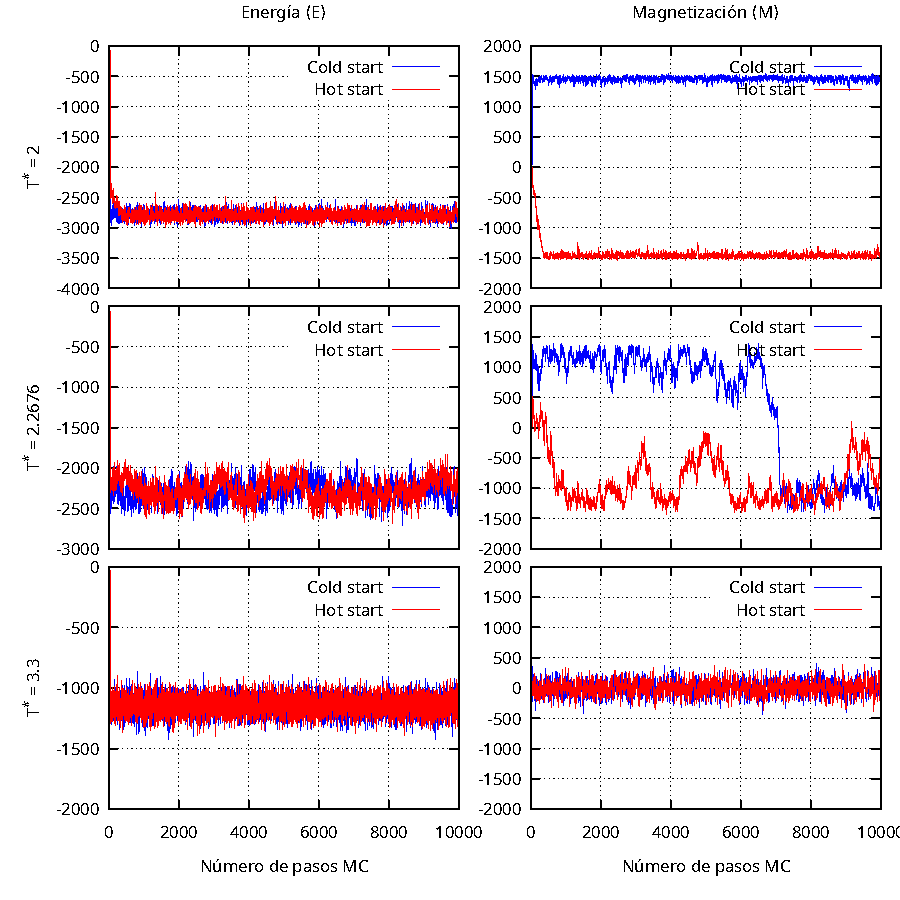
\includegraphics[width = \textwidth]{../img/a.pdf}
    \caption{Valores de $\langle M \rangle$ y $\langle E \rangle$ en función del número de pasos MC.}
    \label{fig:a}
\end{figure}

En la Figura \ref{fig:b} presentamos,\footnote{Inciso b.} como función de la temperatura reducida $T^*$, el valor absoluto de la magnetización por partícula, la energía por partícula, la susceptibilidad y el calor específico. Estimamos todos estos valores por integración MC con $N = 10000$ pasos y un {\it burn in} de 1000 pasos. Hacemos esto para modelos de Ising de tamaños $n = 10$, $n = 20$ y $n = 40$, donde $n$ es el número de partículas por lado. En la Figura \ref{fig:b_bis} presentamos, para discutir posteriormente, un acercamiento de los gráficos de la Figura \ref{fig:b}.

\begin{figure}[h!]
    \centering
    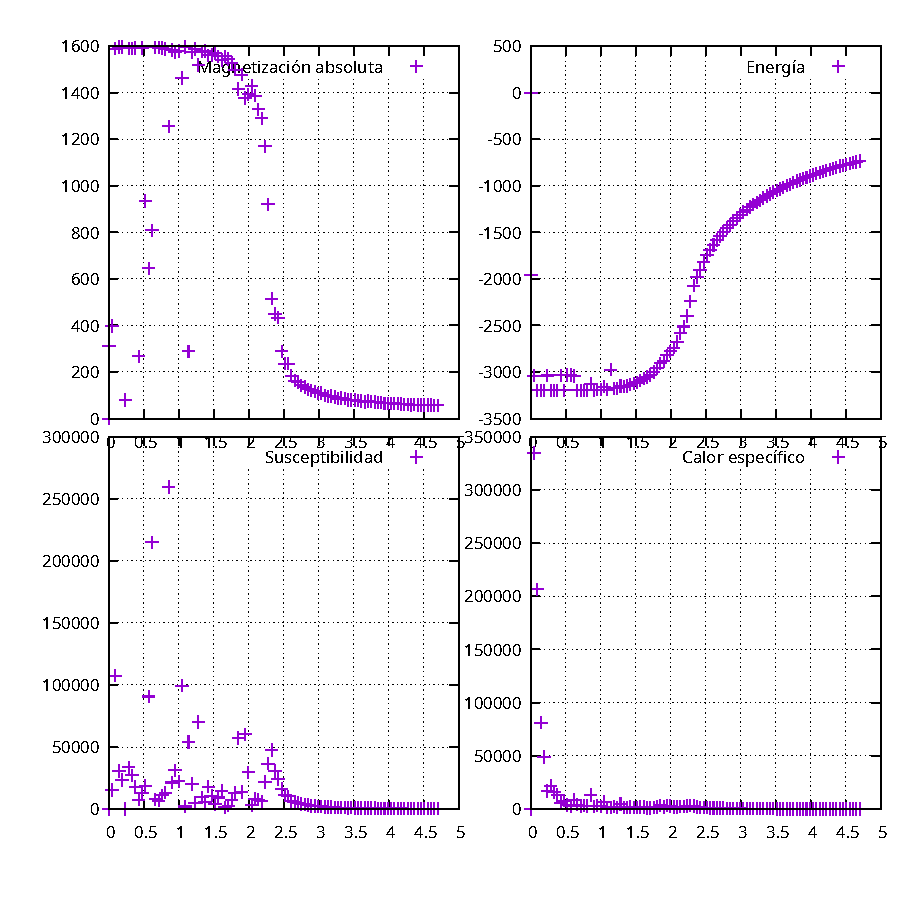
\includegraphics[width = .9\textwidth]{../img/b.pdf}
    \caption{Algunas variables termodinámicas en función de la temperatura reducida $T^*$.}
    \label{fig:b}
\end{figure}

\begin{figure}[h!]
    \centering
    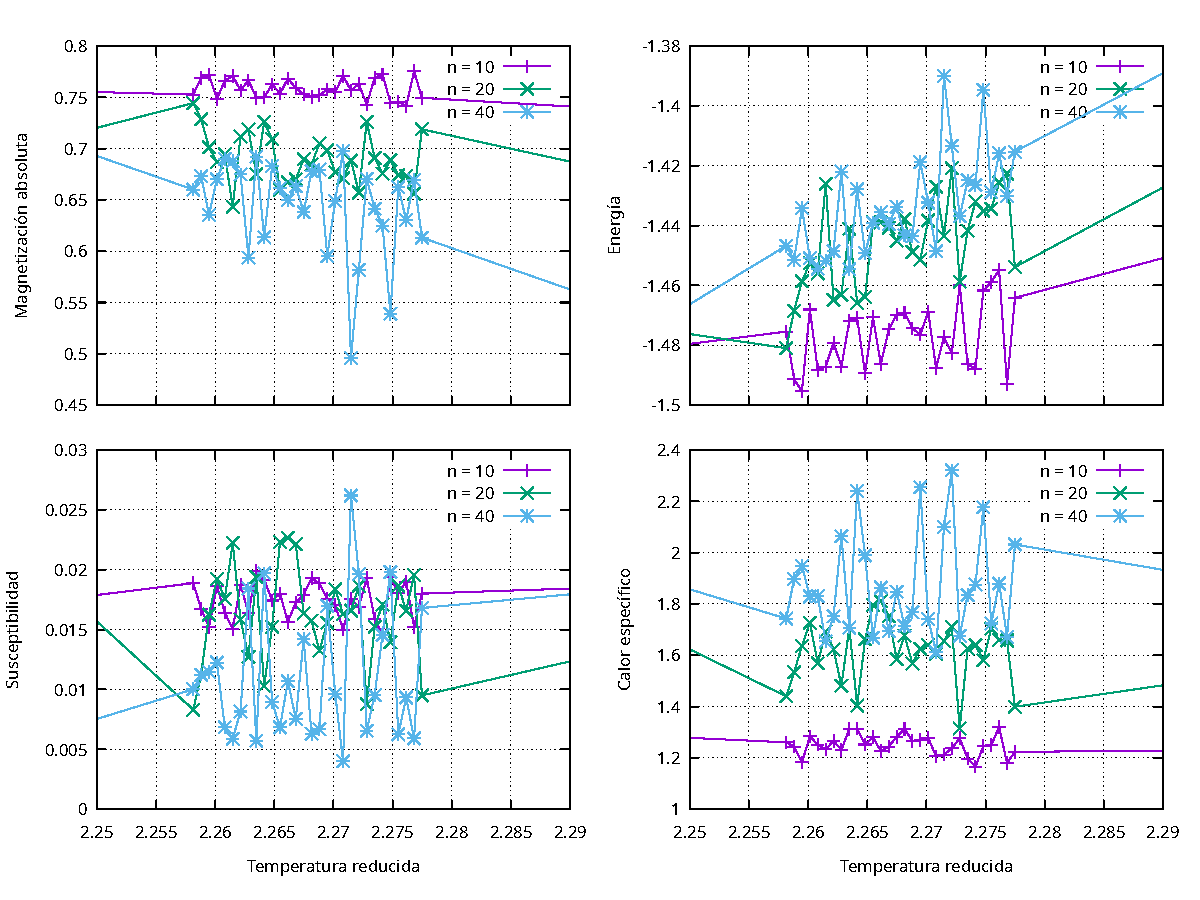
\includegraphics[width = .9\textwidth]{../img/b_bis.pdf}
    \caption{Acercamiento de la Figura \ref{fig:b}.}
    \label{fig:b_bis}
\end{figure}

\newpage

En la Figura \ref{fig:c} presentamos,\footnote{Inciso c.} para dos temperaturas reucidas diferentes (una ligeramente por encima y otra ligeramente por debajo de la temperatura crítica $T_c = 2.2676$), los histogramas de la magnetización en el modelo de Ising de tamaño $40 \times 40$. Para esto, como antes, excluímos un {\it burn in} de 1000 pasos MC y armamos el histograma con los datos de magnetización de $N = 10000$ estados del modelo.

\begin{figure}[h!]
    \centering
    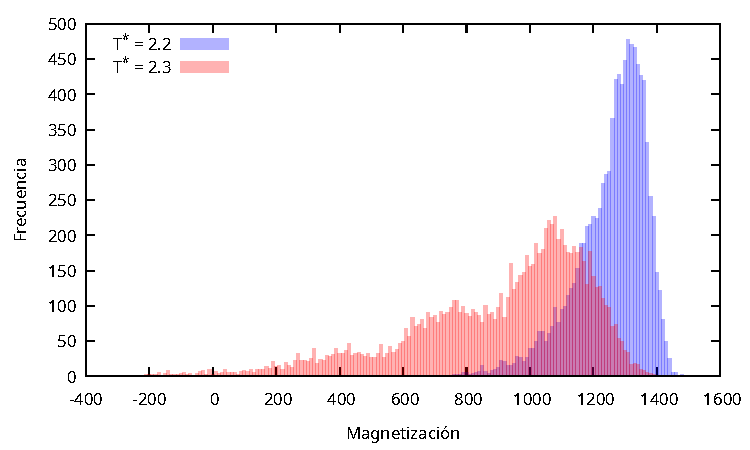
\includegraphics[width = .8\textwidth]{../img/c.pdf}
    \caption{Histogramas de $\langle M \rangle$ a diferentes temperaturas.}
    \label{fig:c}
\end{figure}

En la Figura \ref{fig:d} presentamos,\footnote{Indiso d.} para distintos tamaños de modelo, los {\it cumulantes de Binder}. Calculamos estos valores a partir de datos de magnetización obtenidos por integración MC con {\it burn in} de 1000 pasos y tamaño de muestra de $N = 100000$ pasos MC. Notese el incremente en el número de pasos.

\begin{figure}[h!]
    \centering
    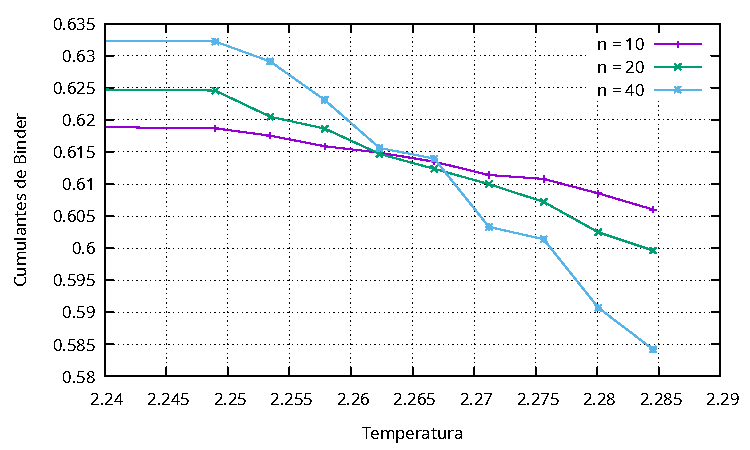
\includegraphics[width = .8\textwidth]{../img/d.pdf}
    \caption{Cumulantes de Binder para modelos de diferentes tamaños.}
    \label{fig:d}
\end{figure}

En la Figura \ref{fig:d_bis} mostramos los valores de $\langle |M| \rangle$ y $\chi$ obtenidos anteriormente por integración MC junto con las funciones $(T_c - T)^\beta$ y $|T - T_c|^{-\gamma}$. Se usan los exponentes críticos $\beta = \frac{1}{8}$ y $\gamma = \frac{7}{4}$ encontrados por Onsager [CITA A ONSAGER].

\begin{figure}[h!]
    \centering
    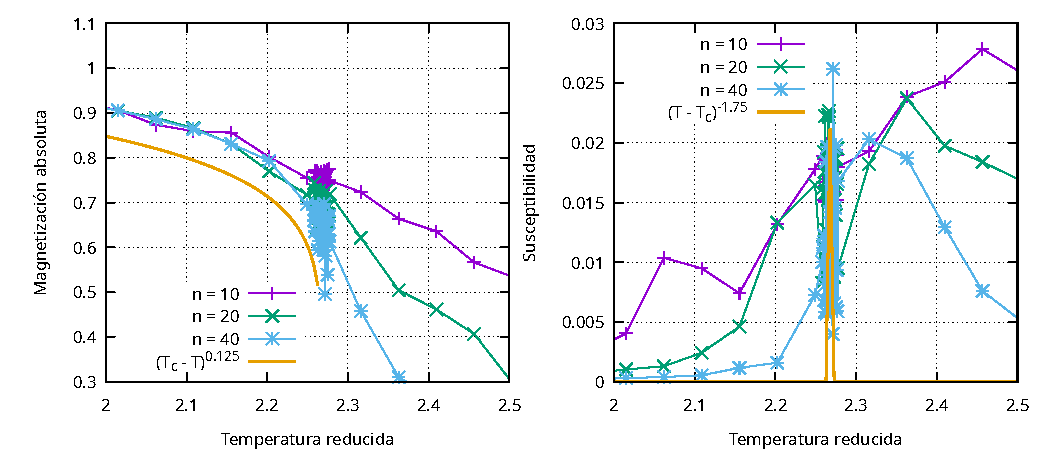
\includegraphics[width = \textwidth]{../img/d_bis.pdf}
    \caption{Exponentes críticos.}
    \label{fig:d_bis}
\end{figure}

Finalmente, en la Figura \ref{fig:e} presentamos las funciones de autocorrelación de la magnetización $|M|$ y energía $E$ calculadas a partir de los estados dados por el método de Metropolis. En función de estos datos, en la Tabla \ref{tab:tau} presentamos cotas para los tiempos de autocorrelación de magnetización $\tau_M$ y energía $\tau_E$.

\begin{figure}[h!]
    \centering
    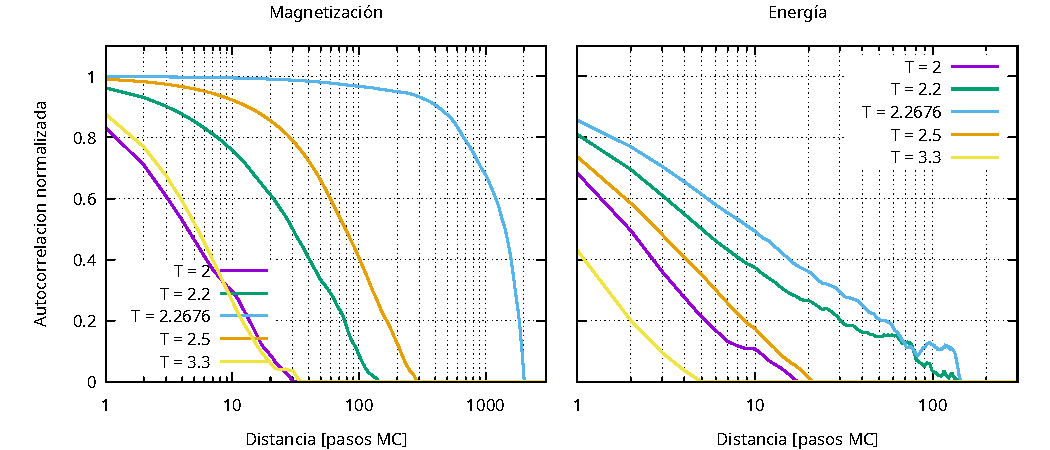
\includegraphics[width = \textwidth]{../img/e.pdf}
    \caption{Funciones de autocorrelación de $|M|$ y $E$.}
    \label{fig:e}
\end{figure}

\newpage

\begin{table}[h!]
    \centering
    \begin{tabular}{c|c|c}
        $T$ & $\tau_M$ & $\tau_E$ \\ \hline
        2 & 7.4 & 3.5 \\
        2.2 & 40.9 & 20.3 \\
        2.2676 & 1179 & 29.7 \\
        2.5 & 96 & 5  \\
        3.3 & 7.5 & 1.3  \\
    \end{tabular}
    \caption{Tiempos de autocorrelación \( \tau_M \) y \( \tau_E \) en función de $T$.}
    \label{tab:tau}
\end{table}

\section{Discusión}

Dividimos esta sección en varias subsecciones porque de otra forma sería muy extensa. La primera de estas subsecciones es, por lejos, la más importante, porque las observaciones que se presentan allí explican (casi por completo) las observaciones que se presentan en las demas subsecciones.

\subsection{Muestreo de $S$ con el método de Metropolis}

Intuitivamente, el muestreo por cadenas de Markov produce una sucesión de variables aleatorias distribuídas aproximadamente según la distribución de Boltzman. Esta distribución depende de la temperatura $T^*$ y asigna probabilidades mas altas a estados de menor energía (ver \cite{phillies2000elementary}). Para temperaturas bajas (por debajo de $T_c$) el resultado de esto es que los sistemas muestreados tienden a tener espines alineados (ya sea {\it up} o {\it down}, el modelo de Ising es simétrico en este sentido). Para temperaturas altas (por encima de $T_c$) ocurre lo contratio: los sistemas muestreados tienden a tener espines aleatorios. Dado que la magnetización depende de la suma de los espines (midiendo, en cierto sentido, la alineación general del sistema), es de esperarse que para temperaturas bajas, sea muy alta, y para temperaturas altas, sea cercana a 0. Esto es lo que se oberva en las gráficas del lado izquierdo de la Figura \ref{fig:a}. Por otro lado, la energía depende de (el negativo de) la suma de los productos de espines cercanos (midiendo, en cierto sentido, la alineación local del sistema), por lo que es de esperarse que sea baja a temperaturas bajas y alta a temperaturas altas, como se observa en las gráficas del lado derecho de la Figura \ref{fig:a}.\\

Hamos mencionado en la Sección \ref{sec:preliminares} que el muestreo por cadenas de Markov produce un {\it burn in} que debe desecharse, esto se ve al inicio de las gráficas de la Figura \ref{fig:a} pero es más notorio a temperaturas bajas con un {\it hot start} (pues el estado inicial es desordenado y debe ordenarse) o temperaturas altas con un {\it cold start} (pues el estado inicial es ordenado y debe desordenarse).\\ %En la Figura \ref{fig:a_bis} mostramos un acercamiento de la Figura \ref{fig:a} en estos dos casos.

Sobre el final de la Sección \ref{sec:preliminares} mencionamos también que en distribuciones bimodales donde la probabilidad se concentra en regiones cercanas a las modas y separadas por valles de probabilidad baja, el muestreo por cadenas de Markov puede tardar mucho en producir una muestra aproximadamente independiente. Este es el caso de la distribución de Boltzmann para el modelo de Ising a temperaturas por debajo de $T_c$. Esta es una observación sumamente interesante, porque al ver las gráficas de la Figura \ref{fig:a} correspondientes a $T^* = 2.2676$, uno podría sospechar que exhiben un comportamiento no deseado, y que debería ocurrir algo como lo que ocurre en las gráficas correspondientes a $T^* = 2$. Sin embargo, es todo lo contrario. Los datos de magnetización en $T^*= 2$ muestran que la cadena de Markov con la cual muestreamos los estados para la integración MC se estanca: el {\it cold start} se implementó como el estado con todos los espines {\it up}, y la cadena de Markov generada a partir de este estado se estancó allí, produciendo una sucesión de estados similares, mientras que en realidad, los estados generalmente alineados {\it up} son igual de probables que los estados generalmente alineados {\it down}. Análogamente, el {\it hot start} dió lugar a una cadena de estados que terminaron alineandose mayoritariamente {\it down} (aunque podrían haber sido {\it up}) y se estancaron allí.

Las gráficas correspondientes a $T^* = 2.2676$, en cambio, exhiben un comportamiento mas deseable. Si bien las cadenas de Markov que generan los estados se estancan en regiones cercanas a una de las modas, eventualmente son capaces de saltar a la región cercana a la otra moda. Esto nos dice que para $T_c$, a pesar de que la distribución de Boltzman del modelo de Ising es bimodal, las regiones de alta probabilidad cercanas a cada moda estan relativamente cerca. Al menos, suficiente para que la distribución de la propuesta de salto $g(\; \cdot \mid x)$ pueda saltar de una a otra.\\

Esta observación nos conduce a una sugerencia para evitar el problema: cambiar la distribución de $g$. En nuestro caso, la probabilidad $g(\; \cdot \mid x)$ es uniforme sobre el conjunto $X = \{x' \in S : d_H(x', x) = 1 \}$, donde $d_H$ es la distancia de Hamming. Esto hace extremadamente improbable que la cadena de Markov pueda saltar de la región cercana a una moda hasta la región cercan a la otra moda cuando la temperatura es baja. Un algoritmo diferente, como por ejemplo, proponer varios flips simultaneos y {\it luego} calcular $\Delta E$, representaría una distribución $g$ mas amplia, por lo que podría lograr muestras de la distribucioń de Boltzmann en temperaturas cercanas a $T_c$ en menos pasos MC. Por supuesto, esto no soluciona el problema, simplemente lo desplaza. De implementar esta solucioń, el fenómeno que dificulta el muestreo, en lugar de presentarse en $T_c$, se presentaría en alguna otra temperatura menor a $T_c$.

Otra solución para conseguir mejores muestras, tomando ventaja de la simetría del modelo, es generar dos cadenas de Markov $Y$ y $Z$, ambas con un {\it cold start}, una con espines {\it up} y la otra con espines {\it down}, y definir también una sucesión $B$ de variables Bernoulli independientes. Combinando estos 3 procesos aleatorios, obtendríamos una sucesión de variables
\begin{equation}
    W_n =
    \begin{cases}
        Y_n, & B_n = 1\\
        Z_n, & B_n = 0
    \end{cases}
\end{equation}
que contemple ambas regiones.

\subsection{Variables termodinámicas}

En la Figura \ref{fig:b} los resultados son los esperados. A medida que la temperatura aumenta, el promedio de la magnetización absoluta baja y la energía aumenta. Dado que el autor desconoce gran parte de la teoría, es dificil discutir mucho mas sobre la interpretación o el significado de los resultados obtenidos para susceptibilidad y calor específico. Es preciso mencionar también que el autor no muestra, ahora mismo, un interés particular por entender qué representan estas variables, quizás a medida que se instruya en mecánica estadística cambie de parecer. Todo depende de la habilidad de \cite{phillies2000elementary} para motivar este estudio.\\

Por otro lado, el autor si se interesa por los aspectos estocásticos de los resultados en la Figura \ref{fig:b}. Un fenómeno de interesante para observar con respecto a esto, ampliado en la Figura \ref{fig:b_bis}, es la variabilidad en los resultados para temperaturas cercanas a la temperatura crítica. En particular, cómo se relacionan la amplitud de estas variaciones con el tamaño de modelo: parece variar más cuanto más grande es el modelo. Como ya hemos discutido, la presencia de variaciones se explica por defectos de la estrategia con la que muestreamos el espacio de estados, una mala muestra conduce a una integral MC pobre. Sospechamos que el hecho de que la variabilidad sea mayor para modelos mas grandes se debe al mismo problema: la cadena de Markov que usamos para muestrear la distribución de Boltzmann se estanca en la región cercana a una de las modas y rara vez saltará a la región correspondiente a la otra moda. Para lograr este salto deben ocurrir varios flips de {\it up} a {\it down} (o al revez) mas o menos consecutivamente (sin que ocurran demasiados flips opuestos entre medio), de forma que el sistema pase de estar magnetizado mayoritariamente {\it down} a estar magnetizado mayoritariamente {\it up}. Cuanto más grande es un modelo, más flips (relativamente) consecutivos se requieren para lograr este salto, lo cual hace mas improbable que ocurra. Esto significa que la cadena de Markov pasará más tiempo en la región cercana a una de las modas antes de saltar a la región cercana a la otra moda. Dado que nuestras meustras son de tamaño $N = 10000$ fijo (el mismo para todas las temperaturas), lo anterior implica que la desviación de las integrales MC para modelos más grandes será mayor.\\

En la Figura \ref{fig:c}, también, los resultados son los esperados. Para temperaturas por debajo de la crítica, la magnetización se concentra en valores negativos, lo que nos indica que la cadena de Markov se estanca en la región cercana a una de las modas. Por otro lado, para temperaturas por encima de la crítica, la magnetización se distribuye (aproximadamente) normal al rededor de 0, indicando que la cadena de Markov no se estanca, es capaz de explorar libremente las regiones correspondientes a ambas modas.

\subsection{Estimación de $T_c$}

De la Figura \ref{fig:d} se puede concluír, intuitivamente, que la temperatura crítica debe estar entre 2.2625 y 2.2675. Formalmente, sería necesario estimar la probabilidad de que la temperatura crítica pertenezca a este intervalo en base a la definición de los cumulantes de Binder y su comportamiento a medida que el tamaño del modelo $n \to \infty$. Esto podría ser interesante, pero dejamos este cálculo para más adelante, una vez hayamos estudiado un poco mas sobre mecánica estadística.

\subsection{Autocorrelación y estimación de errores}

Como mencionamos en la Sección \ref{sec:preliminares}, la desviación en la integración Monte Carlo cuando el muestreo no es independiente es mayor que la desviación con muestreo independiente. En el caso de MCMC, la propiedad de Markov permite calcular indicadores como la autocorrelación $A(k)$ o el tiempo de autocorrelación $\tau_a$, que se pueden usar para corregir la desviación de la integral. En la Figura \ref{fig:e} se muestran las autocorrelaciones de la magnetización y la energía. En teoría, estas funciones deberían aproximar exponenciales (con lo cual, en escala logarítimica deberían parecer lineales), sin embargo, no parece ser el caso para la magnetización a temperaturas $T = 2.2$, $T = 2.2676$ y $T = 2.5$. Suponemos que esto se debe a que el comportamiento exponencial emerge a medida que $n \to \infty$, mientras que la Figura \ref{fig:e} se generó en base a resultados para un modelo de tamaño $n = 40$. En la Tabla \ref{tab:tau} se encuentran los tiempos de autocorrelación asociados a las funciones de autocorrelación de la Figura \ref{fig:e} según \cite{janke2009statistical,schachinger2007mcmc}. Estos tiempos indican, como es de esperarse, que existe una autocorrelacioń enorme al muestrear la distribución de Boltzmann para temperaturas cercanas a $T_c$.

\section{Trabajo futuro}

Sería interesante repetir estos mismos experimentos utilizando una distribución $g$ (la distribución de propuestas) diferente a la utilizada en este trabajo. Esto sería con la esperanza de generar un muestreo más eficiente de la distribución de Boltzmann para temperaturas cercanas a $T_c$. Acompañando esta mejora teórica, sería útil reimplementar los algoritmos de este trabajo en CUDA, de forma que sean paralelizables, y, además, continuar estudiando mecánica estadística, pera ganar mas intuición con la cual interpretar los resultados de las simulaciones.\\

Otros objetivos que quedan por cumplir son leer el manual del compilador (opciones de optimización, tratar advertencias como errores, usar varios compiladores para detectar diferentes errores, etc) y aprender el lenguaje de scripting Bash.\\

Todos los códigos para este trabajo se encuentran en \href{https://github.com/santigiordani/labo-4}{este repositorio}.

%Podríamos chusmear tambien https://archive.org/details/springer_10.1007-978-1-4757-4145-2/page/n15/mode/2up

\bibliographystyle{abbrv}
\bibliography{biblio}

\end{document}